\documentclass[12pt]{article}
\usepackage[brazilian]{babel}
\usepackage[utf8]{inputenc}
\usepackage[T1]{fontenc}
\usepackage{newtxtext,newtxmath}
\usepackage{setspace}
\usepackage{graphicx}
\usepackage{amsmath,amssymb}
\usepackage{subfigure}
\usepackage{titlesec}
\usepackage[margin=2.5cm]{geometry}

% Seções numeradas "N. TÍTULO", negrito, mesmo tamanho do corpo (12pt), não centralizado
\titleformat{\section}{\normalfont\bfseries}{\thesection.}{0.5em}{}
\titlespacing*{\section}{0pt}{1.8ex plus .2ex minus .1ex}{1ex}

\begin{document}
\doublespacing

\begin{center}
{\fontsize{14}{17}\selectfont\bfseries E04 -- Circuito RLC Série: Regime Senoidal}\\[1em]
{\fontsize{12}{15}\selectfont Gael Vinícius Maia Sampaio, Jônatas Augusto de Paula, José Guilherme Correia de Menezes, Paulo Otávio Portela Santana, Pedro Diogo Leal Arteiro}\\[0.6em]
{\fontsize{10}{12}\selectfont\itshape
Instituto Tecnológico de Aeronáutica, Laboratório de Física Experimental (FIS-46)\\
Prof. Resp. Argemiro Soares da Silva Sobrinho\\
São José dos Campos, SP, \today}
\end{center}

\vspace{1.2em}

\noindent\textbf{RESUMO}

\noindent Um circuito RLC série ($R=1\,\text{k}\Omega$, $C=0{,}1\,\mu\text{F}$, $L=160\,\text{mH}$) foi excitado em $f=1270\,\text{Hz}$, próximo da ressonância teórica $f_0=1260\pm90\,\text{Hz}$, e as tensões complexas $V_1$, $V_2$, $V_3$ em três nós do circuito foram medidas com um osciloscópio digital, usando a tensão sobre $R$ como referência de fase. A partir delas calculamos os fasores $V_C=V_1-V_2$, $V_L=V_2-V_3$ e $V_R=V_3$, a resistência interna da bobina ($R_{bobina}=130\pm60\,\Omega$, obtida por divisão fasorial $Z_L=V_L/I$ sem comparação com multímetro, que não foi medido nesta sessão) e as potências dissipadas em cada componente. Os módulos medidos de $V_L$ e $V_C$ concordam com a teoria dentro da incerteza, consistente com a operação próxima da ressonância e com um circuito predominantemente resistivo nessa frequência. As fases calculadas de $V_L$ e $V_C$, no entanto, apresentaram sinal invertido em cerca de $180^\circ$ em relação ao esperado teoricamente, um erro sistemático discutido abertamente no texto e atribuído à polaridade das pontas de prova, não a um erro aleatório de medida, já que a resistência interna derivada da bobina permanece positiva e fisicamente razoável independentemente dessa inversão.

\section{RESULTADOS E DISCUSSÃO}

Um circuito RLC série alimentado por uma fonte senoidal $v(t)=V_0\cos(\omega t)$ responde, em regime estacionário, com uma corrente $i(t)=I_0\cos(\omega t-\theta)$. Usando a notação fasorial complexa $v(t)=\text{Re}(Ve^{j\omega t})$, $i(t)=\text{Re}(Ie^{j\omega t})$, a impedância total do circuito é $Z=R+j(X_L-X_C)$, com reatância indutiva $X_L=\omega L$ e capacitiva $X_C=1/(\omega C)$ \cite{Nussenzveig1997,Halliday2013}. No diagrama fasorial, a tensão sobre o resistor $V_R$ está em fase com a corrente $I$, a tensão sobre o indutor $V_L$ está adiantada de $\pi/2$ em relação a $I$ e a tensão sobre o capacitor $V_C$ está atrasada de $\pi/2$ em relação a $I$; se $|V_L|>|V_C|$ o circuito é predominantemente indutivo, se $|V_L|<|V_C|$ é predominantemente capacitivo, e próximo da frequência de ressonância $f_0=1/(2\pi\sqrt{LC})$ os dois módulos se aproximam e o circuito se torna predominantemente resistivo \cite{Nussenzveig1997,Halliday2013}.

O circuito montado (Figura 4 do roteiro da disciplina) tem, em série, o gerador de funções (com resistência interna $r_g=50\,\Omega$), o capacitor $C$ entre os nós 1 e 2, o indutor real -- modelado como resistência interna $R_{bobina}$ em série com uma indutância ideal $L$ -- entre os nós 2 e 3, e o resistor $R$ entre o nó 3 e o terra. A amplitude do gerador foi ajustada para $20\,\text{Vpp}$ e a frequência para $1270\,\text{Hz}$ (aproximadamente a ressonância teórica), valor confirmado de forma independente pela leitura automática de frequência do próprio osciloscópio Tektronix TBS 1052B-EDU nas duas capturas de tela utilizadas. Com a ponta de prova do canal 2, referenciada ao canal 1 (tensão $V_3$ sobre $R$, tomada como referência de fase, $\phi=0^\circ$), foram medidos o módulo (tensão pico a pico) e a fase dos nós $V_1$ e $V_2$; a Tabela~\ref{tab:brutos} apresenta os dados brutos assim obtidos. A planilha de coleta não registra incerteza de leitura; na ausência de uma medida de cursor documentada, adotamos uma incerteza nominal típica do osciloscópio (exatidão vertical de $\pm3\%$ do valor lido, com piso de $0{,}1\,\text{Vpp}$, e resolução de fase de $\pm1^\circ$), de acordo com o datasheet do fabricante \cite{Tektronix2016}, deixando explícito que se trata de uma suposição. O roteiro também não especifica as tolerâncias dos componentes; adotamos tolerâncias nominais típicas de catálogo ($R\pm5\%$, $C\pm10\%$, $L\pm10\%$), igualmente como suposição.

\begin{table}[htb]
	\caption{\label{tab:brutos} Dados brutos: módulo (tensão pico a pico) e fase dos nós $V_1$, $V_2$, $V_3$, medidos com o canal 2 do osciloscópio referenciado ao canal 1 ($V_3$, fase de referência). Incertezas nominais do instrumento, ver texto.}
	\centering
	\begin{tabular}{ccc}
		\hline\hline
		Grandeza & Módulo (Vpp) & Fase (\textdegree) \\ \hline
		$V_1$ & $19{,}2\pm0{,}6$ & $-1{,}4\pm1{,}0$ \\
		$V_2$ & $28{,}0\pm0{,}8$ & $-47{,}5\pm1{,}0$ \\
		$V_3$ & $16{,}8\pm0{,}5$ & $0{,}0\pm1{,}0$ \\ \hline\hline
	\end{tabular}
\end{table}

A partir da Tabela~\ref{tab:brutos}, calculamos os fasores complexos $V_C=V_1-V_2$, $V_L=V_2-V_3$ e $V_R=V_3$ (subtração de partes real e imaginária, com incerteza propagada pela regra usual de propagação de erros \cite{Vuolo1996}), apresentados na Tabela~\ref{tab:fasores}. A Figura~\ref{fig:capturas} mostra as duas capturas de tela do osciloscópio usadas para obter $V_1$ e $V_2$; a fase de $V_2$ lida diretamente na captura de tela [painel (b)] é $-46{,}7^\circ$, enquanto o valor anotado na planilha de dados foi $-47{,}5^\circ$ -- uma diferença de $0{,}8^\circ$, menor que a incerteza de leitura adotada mas ainda assim uma discrepância real entre o valor fotografado e o valor registrado, possivelmente por um pequeno reajuste do cursor entre a anotação e a captura; mantivemos o valor da planilha nos cálculos, por ser o registrado oficialmente.

\begin{figure}[htp]
	\centering
	\subfigure[$V_1$: Ch1$=V_3$, Ch2$=V_1$]{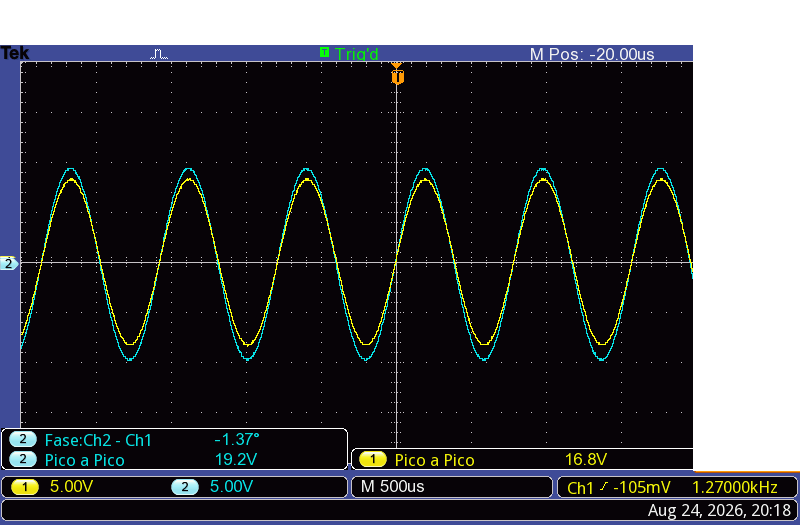
\includegraphics[width=0.48\linewidth]{figs/posicao_1_3_cortada.png}}
	\subfigure[$V_2$: Ch1$=V_3$, Ch2$=V_2$]{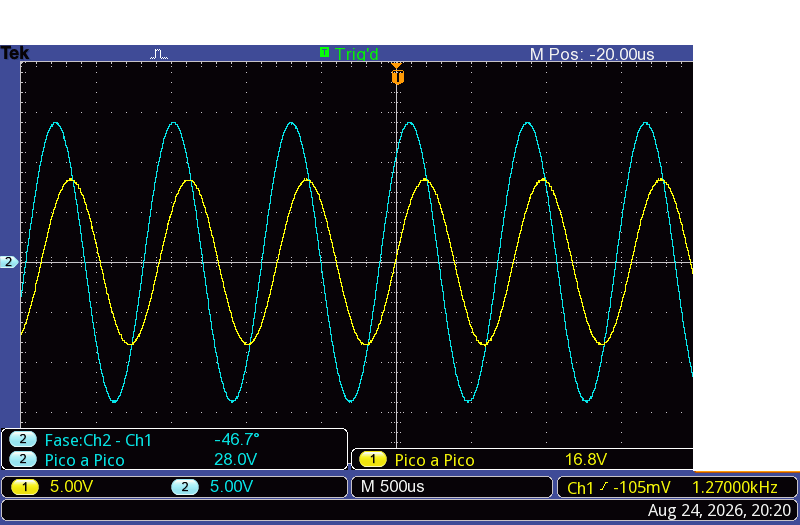
\includegraphics[width=0.48\linewidth]{figs/posicao_2_3_cortada.png}}
	\caption{\label{fig:capturas} Telas do osciloscópio TBS 1052B-EDU (traço amarelo: Ch1$=V_3$, referência de fase; traço ciano: Ch2$=V_1$ em (a) e Ch2$=V_2$ em (b)), com os quadros de leitura de módulo (pico a pico) e fase, além da base de tempo e a frequência medida ($1{,}27000\,\text{kHz}$).}
\end{figure}

\begin{table}[htb]
	\caption{\label{tab:fasores} Fasores derivados $V_C=V_1-V_2$, $V_L=V_2-V_3$ e $V_R=V_3$ (item 2.3 do roteiro). $^\dagger$Fase calculada diretamente da subtração de fasores; ver discussão no texto sobre a inversão de sinal aparente de $V_L$ e $V_C$ em relação à teoria.}
	\centering
	\begin{tabular}{ccc}
		\hline\hline
		Grandeza & Módulo (Vpp) & Fase$^\dagger$ (\textdegree) \\ \hline
		$V_C$ & $20{,}2\pm0{,}8$ & $89\pm3$ \\
		$V_L$ & $20{,}8\pm0{,}8$ & $-84\pm2$ \\
		$V_R$ & $16{,}8\pm0{,}5$ & $0{,}0\pm1{,}0$ \\ \hline\hline
	\end{tabular}
\end{table}

A Figura~\ref{fig:fasores}(a) mostra o diagrama de fasores de $V_R$, $V_L$ e $V_C$ (item 2.4 do roteiro), comparando os valores medidos com os previstos teoricamente a partir de $R$, $L$, $C$ nominais e da corrente de referência $I=V_R/R$; a Figura~\ref{fig:fasores}(b) mostra a cadeia de nós medidos $V_3\to V_2\to V_1$. Os módulos de $V_L$ e $V_C$ concordam com a teoria dentro de poucas vezes a incerteza combinada (resíduos de $-0{,}7\pm2{,}6\,\text{Vpp}$ e $-0{,}9\pm2{,}6\,\text{Vpp}$, respectivamente -- ver Figura~\ref{fig:residuos}(a) e discussão adiante). As \emph{fases} calculadas, porém, saem com sinal oposto ao esperado: a teoria prevê $V_L$ adiantado de $+90^\circ$ e $V_C$ atrasado de $-90^\circ$ em relação a $I$, mas obtivemos $-84\pm2^\circ$ e $+89\pm3^\circ$, respectivamente -- um espelhamento de quase $180^\circ$ em torno do eixo real, e não um desvio aleatório pequeno. Esse tipo de discrepância sistemática -- inversão de sinal -- deve ser discutido abertamente: como ambos os fasores derivados ($V_L$ e $V_C$) invertem o sinal da mesma forma, e como os módulos medidos concordam bem com a teoria, a causa mais provável não é um erro de módulo ou de conexão do circuito, mas sim uma inversão de polaridade na ponta de prova do canal 2 (ou na forma como a leitura "Fase:Ch2$-$Ch1" do osciloscópio resolve o sinal), afetando igualmente as duas capturas de tela usadas para obter $V_1$ e $V_2$. Essa hipótese é reforçada adiante pelo cálculo da resistência interna da bobina, que resulta positivo e fisicamente razoável independentemente dessa ambiguidade de sinal.

\begin{figure}[htp]
	\centering
	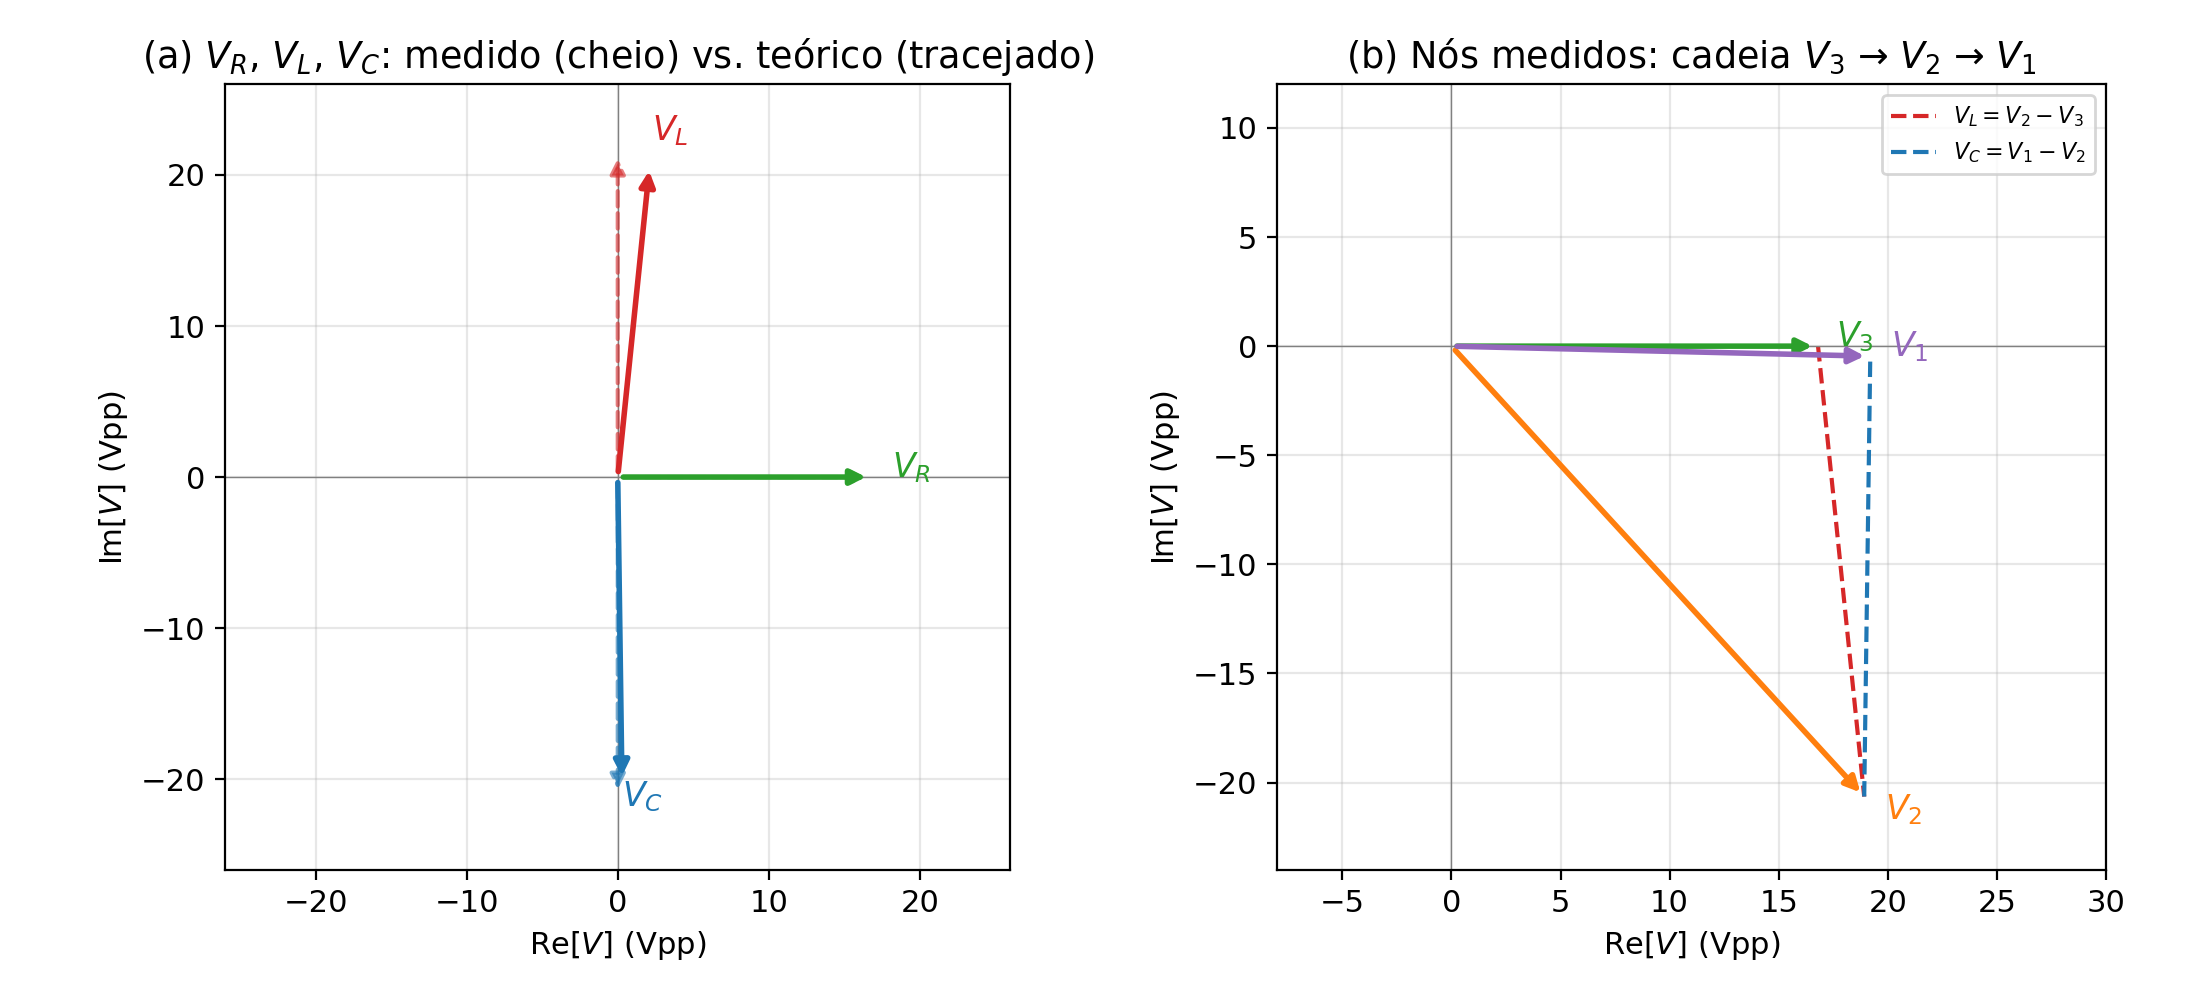
\includegraphics[width=\linewidth]{figs/fasores.png}
	\caption{\label{fig:fasores} (a) Diagrama de fasores de $V_R$, $V_L$ e $V_C$ com origem comum: medido (vetor cheio) contra teórico (tracejado), com a fase de $V_L$ e $V_C$ já espelhada para comparação direta (ver discussão no texto). (b) Nós medidos $V_1$, $V_2$, $V_3$ e a cadeia $V_3\to V_2\to V_1$ no plano complexo.}
\end{figure}

A resistência interna da bobina foi calculada a partir da impedância complexa do ramo do indutor, $Z_L=V_L/I$, com $I=V_R/R$ a corrente de referência do circuito; $R_{bobina}=\text{Re}(Z_L)$. \textbf{Não houve medição de multímetro para a bobina nesta sessão} -- o valor abaixo é inteiramente derivado dos dados de corrente alternada, sem uma comparação direta disponível, ao contrário do que pede o item 2.5 do roteiro. Obtivemos $R_{bobina}=130\pm60\,\Omega$, um valor positivo e da ordem de grandeza esperada para a resistência do fio de cobre enrolado em um indutor de $160\,\text{mH}$ (tipicamente dezenas a poucas centenas de ohms, dependendo da bitola do fio e do número de espiras), portanto fisicamente plausível. A parte imaginária de $Z_L$ resulta em $X_{L,\text{medido}}=-1230\pm90\,\Omega$, com o mesmo sinal invertido discutido acima; se espelhada, $+1230\pm90\,\Omega$ concorda muito bem com o valor teórico $X_L=1280\pm130\,\Omega$, o que reforça a hipótese de inversão de sinal (o cálculo de $R_{bobina}$, por depender apenas da parte real de $Z_L$, não é afetado por essa ambiguidade). A Tabela~\ref{tab:potencias} resume $Z_L$, $R_{bobina}$ e as potências dissipadas em cada componente, obtidas convertendo os módulos de pico a pico para valor eficaz ($V_{rms}=V_{pp}/(2\sqrt2)$): $P_R=I_{rms}^2R$, $P_L=I_{rms}^2R_{bobina}$ e $P_C=0$ (idealização de capacitor ideal, que não dissipa potência ativa).

\begin{table}[htb]
	\caption{\label{tab:potencias} Impedância do ramo do indutor, resistência interna da bobina e potências dissipadas. $I_{rms}=5{,}94\pm0{,}35\,\text{mA}$.}
	\centering
	\begin{tabular}{cc}
		\hline\hline
		Grandeza & Valor \\ \hline
		$\text{Re}(Z_L)=R_{bobina}$ & $130\pm60\,\Omega$ \\
		$\text{Im}(Z_L)=X_{L,\text{medido}}$ & $-1230\pm90\,\Omega$ \\
		$X_L$ teórico & $1280\pm130\,\Omega$ \\
		$P_R$ & $35\pm3\,\text{mW}$ \\
		$P_L$ & $4\pm2\,\text{mW}$ \\
		$P_C$ & $0\,\text{mW}$ (ideal) \\ \hline\hline
	\end{tabular}
\end{table}

Quanto à natureza da impedância total na frequência medida (item 2.7 do roteiro): comparando os módulos medidos, $|V_L|-|V_C|=0{,}6\pm0{,}5\,\text{Vpp}$, estatisticamente compatível com zero dentro de aproximadamente $1$ desvio padrão; da mesma forma, $X_L$ teórico ($1280\pm130\,\Omega$) e $X_C$ teórico ($1250\pm130\,\Omega$) são indistinguíveis dentro da incerteza, e a frequência de operação $f=1270{,}0\pm1{,}3\,\text{Hz}$ está a menos de um desvio padrão de $f_0=1260\pm90\,\text{Hz}$. O circuito está, portanto, operando muito próximo da ressonância, com caráter predominantemente resistivo; o pequeno excesso central de $|V_L|$ sobre $|V_C|$ é consistente com $f$ estar ligeiramente acima de $f_0$, região em que o circuito é discretamente indutivo, embora essa diferença não seja estatisticamente significativa com os dados coletados.

Para uma análise de resíduos mais completa, construímos um modelo teórico ancorado em $V_R$ \emph{medido} (e não na amplitude nominal de $20\,\text{Vpp}$ configurada no gerador): o gerador de funções calibra sua amplitude de painel assumindo uma carga de $50\,\Omega$, mas a carga real deste circuito (módulo de impedância da ordem de $1$--$1{,}3\,\text{k}\Omega$) é muito maior, de modo que a força eletromotriz real de circuito aberto do gerador pode diferir substancialmente do valor nominal do painel -- uma fonte de incerteza sistemática não quantificada, que preferimos evitar ancorando o modelo em $V_R$ medido. A partir daí, $V_{L,\text{teo}}=V_R(X_L/R)$ a $+90^\circ$ e $V_{C,\text{teo}}=V_R(X_C/R)$ a $-90^\circ$, dando $V_{L,\text{teo}}=21{,}4\pm2{,}5\,\text{Vpp}$ e $V_{C,\text{teo}}=21{,}1\pm2{,}4\,\text{Vpp}$. A Figura~\ref{fig:residuos} mostra os resíduos (medido$-$teórico) de módulo e de fase (esta última já com o sinal espelhado, conforme discutido). Os resíduos de módulo são pequenos e compatíveis com zero dentro da incerteza combinada; os resíduos de fase corrigida também são majoritariamente compatíveis com zero, com uma leve tendência de $-5{,}9\pm2{,}2^\circ$ para $V_L$, plausivelmente associada a uma pequena defasagem adicional introduzida pela resistência interna real da bobina $R_{bobina}$ (que o modelo teórico ideal, com $L$ puro, não inclui).

\begin{figure}[htp]
	\centering
	
\includegraphics[width=\linewidth]{figs/residuos.png}
	\caption{\label{fig:residuos} Resíduos entre valores medidos e o modelo teórico ancorado em $V_R$: (a) módulo de $V_L$ e $V_C$; (b) fase de $V_L$ e $V_C$, já com o sinal espelhado para comparação direta com a teoria (ver discussão no texto). $V_R$ é a própria referência por construção e não entra neste gráfico.}
\end{figure}

\section{CONCLUSÃO}

Medimos os fasores de tensão em três nós de um circuito RLC série operando a $1270\,\text{Hz}$, próximo da ressonância teórica ($f_0=1260\pm90\,\text{Hz}$), e derivamos $V_C$, $V_L$ e $V_R$, a resistência interna da bobina ($R_{bobina}=130\pm60\,\Omega$, fisicamente plausível, mas sem comparação com multímetro por falta de medição nesta sessão) e as potências dissipadas ($P_R=35\pm3\,\text{mW}$, $P_L=4\pm2\,\text{mW}$, $P_C=0$). Os módulos de $V_L$ e $V_C$ concordam com o modelo teórico dentro da incerteza, e a comparação $|V_L|\approx|V_C|$ confirma que o circuito opera de forma predominantemente resistiva na frequência escolhida, como esperado próximo da ressonância. Identificamos e discutimos abertamente uma inversão sistemática de aproximadamente $180^\circ$ no sinal da fase calculada de $V_L$ e $V_C$ em relação à teoria -- não um erro aleatório, já que afeta os dois fasores de forma consistente e não compromete os módulos nem a resistência interna derivada --, atribuída à polaridade da ponta de prova do canal 2 do osciloscópio. Também observamos uma pequena discrepância de $0{,}8^\circ$ entre a fase de $V_2$ registrada na planilha e a lida na captura de tela correspondente, dentro da incerteza de leitura adotada. Este trabalho ilustra tanto a aplicação do método fasorial à análise de circuitos RLC quanto a importância de identificar e discutir explicitamente discrepâncias sistemáticas de medida, em vez de ocultá-las.

\section{REFERÊNCIAS BIBLIOGRÁFICAS}
\renewcommand{\refname}{}
\bibliographystyle{unsrt}
\bibliography{library}

\end{document}
